% Now that we understand logical clocks and the partial ordering of events in a
% distributed systems, we'll switch gears and talk about the Chandy Lamport
% snaphshot algorithm. Explain what a snapshot is. Explain how the notion is
% very deeply tied to the idea of logical time.
\frozen{}

\tikzstyle{vert}=[circle, minimum width=1cm, draw, thick]

% Our system is composed of a finite set of processes and channels represented
% as vertices and edges in a directed graph. Channels are assumed to
%
%   (a) have infinite buffers, and
%   (b) be error-free, and
%   (c) deliver messages FIFO.
%
% Channel delay is arbitrary but finite.
\begin{frame}
  \begin{center}
    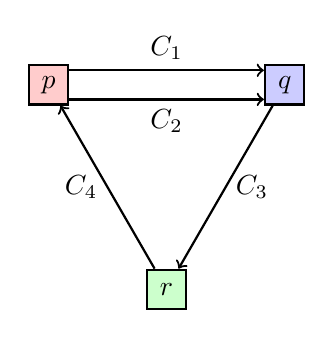
\begin{tikzpicture}
      \node[vert, fill=red!20]   (p) at (0, 0)  {$p$};
      \node[vert, fill=blue!20]  (q) at (0:3)   {$q$};
      \node[vert, fill=green!20] (r) at (300:3) {$r$};
      \draw[thick, ->] (p.35)  -- node[above]{$C_1$} (q.145);
      \draw[thick, ->] (p.325) -- node[below]{$C_2$} (q.215);
      \draw[thick, ->] (q)     -- node[right]{$C_3$} (r);
        \draw[thick, ->] (r)   -- node[left ]{$C_4$} (p);
    \end{tikzpicture}
  \end{center}
\end{frame}

\tikzstyle{vert}=[
  inner sep=0cm,
  minimum width=0.5cm,
  minimum height=0.5cm,
  draw,
  thick,
]
\tikzstyle{p}=[circle, vert]
\tikzstyle{q}=[vert]

\newcommand{\barbell}[6]{
  \node[p]                     (p#1) at #2 {#3};
  \node[q, right=0.5cm of p#1] (q#1)       {#4};
  \draw[->, thick] (p#1.35)  -- node[above]{#5} (q#1.150);
  \draw[<-, thick] (p#1.325) -- node[below]{#6} (q#1.210);

  \node (c#1) at ($(p#1)!0.5!(q#1)$) {};

  \node[above=0.35cm of c#1] (n#1) {};
  \node[right=0.25cm of q#1] (e#1) {};
  \node[below=0.35cm of c#1] (s#1) {};
  \node[left =0.25cm of p#1] (w#1) {};

  \node[above=0.35cm of e#1] (ne#1) {};
  \node[below=0.35cm of e#1] (se#1) {};
  \node[below=0.35cm of w#1] (sw#1) {};
  \node[above=0.35cm of w#1] (nw#1) {};
}

\newcommand{\tkn}{\ensuremath{\bullet}}
\newcommand{\blt}{\ensuremath{\textcolor{red!75}{\bullet}}}
\newcommand{\bbt}{\blt\blt}

\newcommand{\onetoken}{
  \barbell{1}{(0,  0)}{\blt}{    }{    }{    };
  \barbell{2}{(5,  0)}{    }{    }{\blt}{    };
  \barbell{3}{(5, -3)}{    }{\blt}{    }{    };
  \barbell{4}{(0, -3)}{    }{    }{    }{\blt};
  \draw[ultra thick, ->, black] (e1) -- (w2);
  \draw[ultra thick, ->, red  ] (s2) -- (n3);
  \draw[ultra thick, ->, green] (w3) -- (e4);
  \draw[ultra thick, ->, blue ] (n4) -- (s1);
}

% This is a concise way to describe the set of all global system states and the
% set of all computations. Here, each process and each channel has two states.
% Each vertex in this graph of graphs is a global system state. Every finite
% length walk starting from the initial state is a computation. This example is
% a single-token system.
\begin{frame}
  \begin{center}
    \begin{tikzpicture}
      \onetoken
    \end{tikzpicture}
  \end{center}
\end{frame}

\begin{frame}{Distributed System Model}
  A \emph{process} $p$ is a set of states $S$, an initial state $s$, and a set
  of events $E$.
  \[
    p \triangleq (S, s, E)
  \]

  \pause

  An \emph{event} $e \in E$ is defined by a process $p$, the state $s$ and $s'$
  of $p$ before and after $e$, the channel $(c | \bot)$ modified by $e$, and
  the message $(M | \bot)$ sent or received on $c$.
  \[
    e \triangleq (p, s, s', (M | \bot), (c | \bot))
  \]

  \pause

  A \emph{global state} is a set of process and channel states. The
  \emph{initial global state} has all processes in their initial states and all
  channels empty. A \emph{computation of the system} is a sequence of events.
  % Note that there are the intuitive restrictions on computations. Not all
  % sequences of events form a computation.
\end{frame}

\newcommand{\twotoken}{
    \barbell{01}{(+0, +0)}{\blt}{\blt}{    }{    };
    \barbell{02}{(+1, +1)}{\blt}{    }{    }{\blt};
    \barbell{03}{(+1, -1)}{    }{\blt}{\blt}{    };
    \barbell{04}{(+2, +2)}{\bbt}{    }{    }{    };
    \barbell{05}{(+2, +0)}{    }{    }{\blt}{\blt};
    \barbell{06}{(+2, -2)}{    }{\bbt}{    }{    };
    \barbell{07}{(+3, +2)}{\blt}{    }{\blt}{    };
    \barbell{08}{(+3, -2)}{    }{\blt}{    }{\blt};
    \barbell{09}{(+4, +1)}{    }{    }{    }{\bbt};
    \barbell{10}{(+4, -1)}{    }{    }{\bbt}{    };
    \draw[ultra thick, ->, black] (e01) -- (w02);
    \draw[ultra thick, ->, blue ] (e01) -- (w03);
    \draw[ultra thick, ->, green] (e02) -- (w04);
    \draw[ultra thick, ->, blue ] (e02) -- (w05);
    \draw[ultra thick, ->, black] (e03) -- (w05);
    \draw[ultra thick, ->, red  ] (e03) -- (w06);
    \draw[ultra thick, ->, blue ] (e04) -- (w07);
    \draw[ultra thick, ->, green] (e05) -- (w07);
    \draw[ultra thick, ->, red  ] (e05) -- (w08);
    \draw[ultra thick, ->, black] (e06) -- (w08);
    \draw[ultra thick, ->, blue ] (e07) -- (w10);
    \draw[ultra thick, ->, black] (e08) -- (w09);
    \draw[ultra thick, ->, green] (w09) -- (e02);
    \draw[ultra thick, ->, red  ] (w10) -- (e03);
}

\newcommand{\twotokensnap}{
    \barbell{01}{(+0, +0)}{\blt}{\blt}{\tkn    }{    };
    \barbell{02}{(+1, +1)}{\blt}{    }{        }{\blt};
    \barbell{03}{(+1, -1)}{    }{\blt}{\blt\tkn}{    };
    \barbell{04}{(+2, +2)}{\bbt}{    }{        }{    };
    \barbell{05}{(+2, +0)}{    }{    }{\blt\tkn}{\blt};
    \barbell{06}{(+2, -2)}{    }{\bbt}{        }{    };
    \barbell{07}{(+3, +2)}{\blt}{    }{\blt    }{\tkn};
    \barbell{08}{(+3, -2)}{    }{\blt}{        }{\blt};
    \barbell{09}{(+4, +1)}{    }{    }{        }{\bbt};
    \barbell{10}{(+4, -1)}{    }{    }{\bbt    }{    };
    \draw[ultra thick, ->, black] (e01) -- (w02);
    \draw[ultra thick, ->, blue ] (e01) -- (w03);
    \draw[ultra thick, ->, green] (e02) -- (w04);
    \draw[ultra thick, ->, blue ] (e02) -- (w05);
    \draw[ultra thick, ->, black] (e03) -- (w05);
    \draw[ultra thick, ->, red  ] (e03) -- (w06);
    \draw[ultra thick, ->, blue ] (e04) -- (w07);
    \draw[ultra thick, ->, green] (e05) -- (w07);
    \draw[ultra thick, ->, red  ] (e05) -- (w08);
    \draw[ultra thick, ->, black] (e06) -- (w08);
    \draw[ultra thick, ->, blue ] (e07) -- (w10);
    \draw[ultra thick, ->, black] (e08) -- (w09);
    \draw[ultra thick, ->, green] (w09) -- (e02);
    \draw[ultra thick, ->, red  ] (w10) -- (e03);
}

% Here is a double-token system. Unlike the single-token system, this system is
% non-deterministic meaning some states have multiple outgoing edges.
\begin{frame}
  \begin{center}
    \scalebox{0.7}{
      \begin{tikzpicture}[xscale=3, yscale=1.5]
        \twotoken{}
      \end{tikzpicture}
    }
  \end{center}
\end{frame}

% Notice that if we take a snapshot of p in the initial state and a snapshot of
% the upper channel in the next state, our snapshot includes two tokens.
% Similarly, if we take a snapshot of the channel in the first state and a
% snapshot of p in the second state, we have no tokens.
%
% This shows that there is a certain order in which we have to take snapshots.
% We cannot record the state of a sender's channel after the sender's state has
% been recorded and after it has sent a message on its outgoing channel.
\begin{frame}
  \begin{center}
    \begin{tikzpicture}
      \onetoken
    \end{tikzpicture}
  \end{center}
\end{frame}

\begin{frame}{Snapshot Algorithm}
  \textbf{Marker-Sending Rule}. For each process $p$ and for each channel $c$
  away from $p$, $p$ records its state and immediately sends a token along $c$.

  \textbf{Marker-Receiving Rule}. For each process $q$ and for each channel $c$
  into $q$, when $q$ receives a token from $c$,
  \begin{itemize}
    \item If $q$ has not yet recorded its state, it records its state and
      records the state of $c$ as the empty sequence.
    \item If $q$ has recorded its state, it records the state of $c$ as the
      sequence of messages since it recorded its state.
  \end{itemize}
\end{frame}

\tikzstyle{v}=[circle, minimum width=1cm]
\tikzstyle{snapped}=[thick, draw, fill=red!50]
\tikzstyle{transient}=[thick, draw, dashed, fill=red!10]
\tikzstyle{arrow}=[ultra thick, ->]
\tikzstyle{darrow}=[ultra thick, ->, dashed]
\tikzstyle{msg}=[above, sloped]

\newcommand{\av}[1]{\node[v, #1] (a) at (0,  0) {$a$};}
\newcommand{\bv}[1]{\node[v, #1] (b) at (4,  2) {$b$};}
\newcommand{\cv}[1]{\node[v, #1] (c) at (4, -2) {$c$};}
\newcommand{\dv}[1]{\node[v, #1] (d) at (8,  0) {$d$};}
\newcommand{\nodes}[4]{
  \av{#1}
  \bv{#2}
  \cv{#3}
  \dv{#4}
}

\newcommand{\ab}[2]{\draw[#1] (a) to node[msg]{#2} (b);}
\newcommand{\ac}[2]{\draw[#1] (a) to node[msg]{#2} (c);}
\newcommand{\bc}[2]{\draw[#1] (b) to node[msg]{#2} (c);}
\newcommand{\bd}[2]{\draw[#1] (b) to node[msg]{#2} (d);}
\newcommand{\cd}[2]{\draw[#1] (c) to node[msg]{#2} (d);}

\newcommand{\tok}{\textcolor{black}{\bullet}\>}
\newcommand{\pre}{\textcolor{red!20}{\bullet}\>}
\newcommand{\post}{\textcolor{red!50}{\bullet}\>}

\begin{frame}
  \begin{center}
    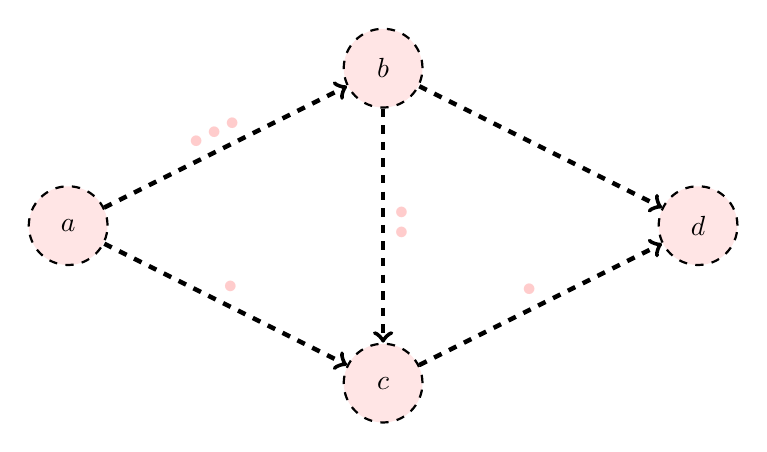
\begin{tikzpicture}
      \nodes{transient}{transient}{transient}{transient}
      \ab{darrow}{$\pre \pre \pre$}
      \ac{darrow}{$\pre$}
      \bc{darrow}{$\pre \pre$}
      \bd{darrow}{$ $}
      \cd{darrow}{$\pre$}
    \end{tikzpicture}
  \end{center}
\end{frame}

\begin{frame}
  \begin{center}
    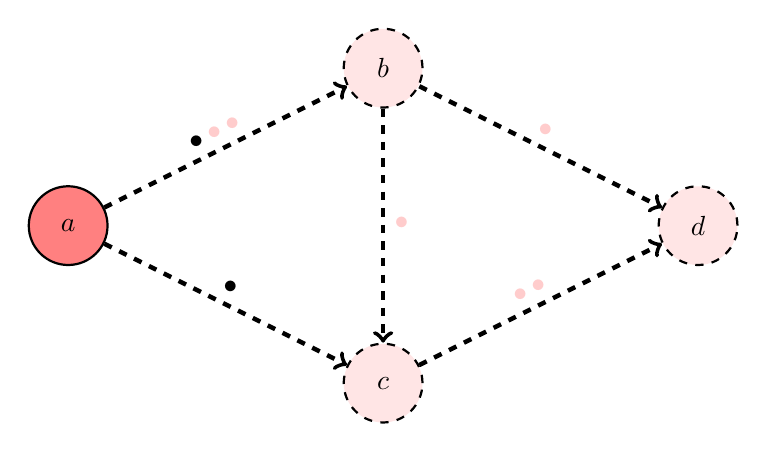
\begin{tikzpicture}
      \nodes{snapped}{transient}{transient}{transient}
      \ab{darrow}{$\tok \pre \pre$}
      \ac{darrow}{$\tok$}
      \bc{darrow}{$\pre$}
      \bd{darrow}{$\pre$}
      \cd{darrow}{$\pre \pre$}
    \end{tikzpicture}
  \end{center}
\end{frame}

\begin{frame}
  \begin{center}
    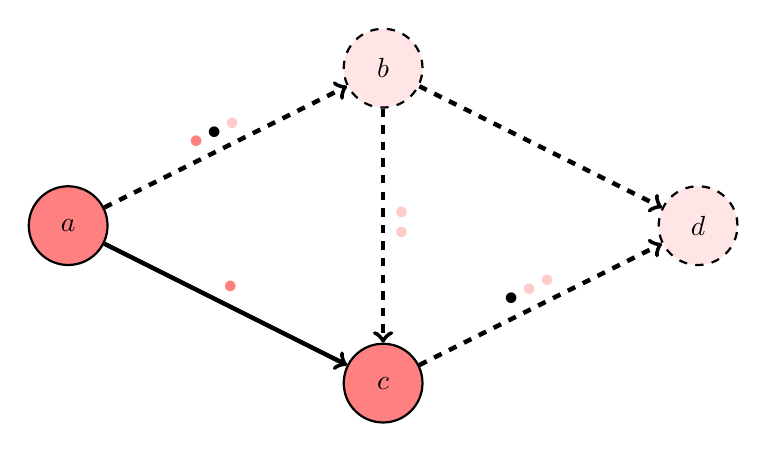
\begin{tikzpicture}
      \nodes{snapped}{transient}{snapped}{transient}
      \ab{darrow}{$\post \tok \pre$}
      \ac{arrow}{$\post$}
      \bc{darrow}{$\pre \pre$}
      \bd{darrow}{$ $}
      \cd{darrow}{$\tok \pre \pre$}
    \end{tikzpicture}
  \end{center}
\end{frame}

\begin{frame}
  \begin{center}
    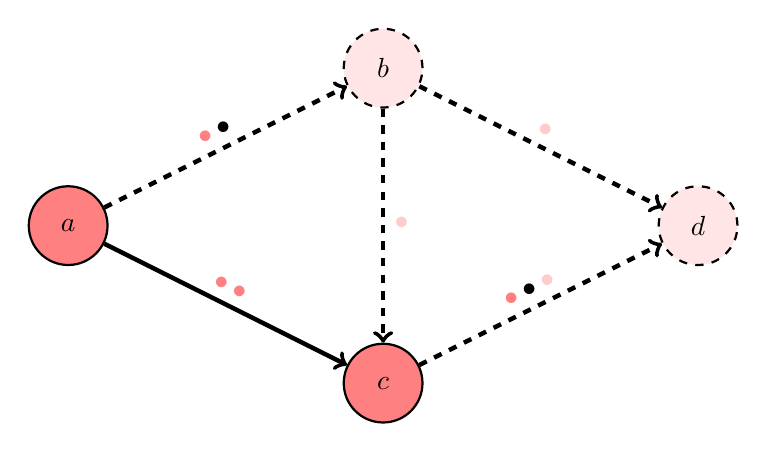
\begin{tikzpicture}
      \nodes{snapped}{transient}{snapped}{transient}
      \ab{darrow}{$\post \tok$}
      \ac{arrow}{$\post \post$}
      \bc{darrow}{$\pre$}
      \bd{darrow}{$\pre$}
      \cd{darrow}{$\post \tok \pre$}
    \end{tikzpicture}
  \end{center}
\end{frame}

\begin{frame}
  \begin{center}
    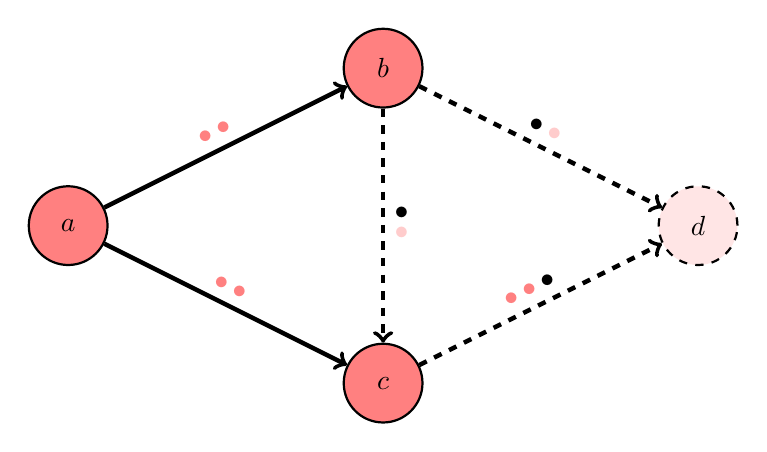
\begin{tikzpicture}
      \nodes{snapped}{snapped}{snapped}{transient}
      \ab{arrow}{$\post \post$}
      \ac{arrow}{$\post \post$}
      \bc{darrow}{$\tok \pre$}
      \bd{darrow}{$\tok \pre$}
      \cd{darrow}{$\post \post \tok$}
    \end{tikzpicture}
  \end{center}
\end{frame}

\begin{frame}
  \begin{center}
    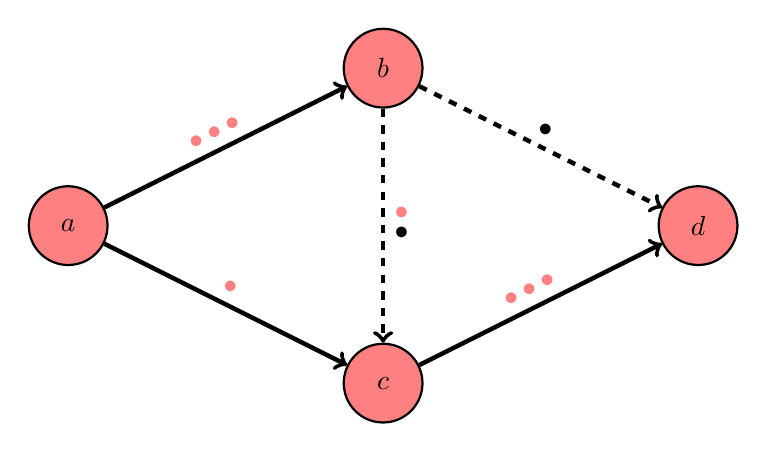
\begin{tikzpicture}
      \nodes{snapped}{snapped}{snapped}{snapped}
      \ab{arrow}{$\post \post \post$}
      \ac{arrow}{$\post$}
      \bc{darrow}{$\post \tok$}
      \bd{darrow}{$\tok$}
      \cd{arrow}{$\post \post \post$}
    \end{tikzpicture}
  \end{center}
\end{frame}

\begin{frame}
  \begin{center}
    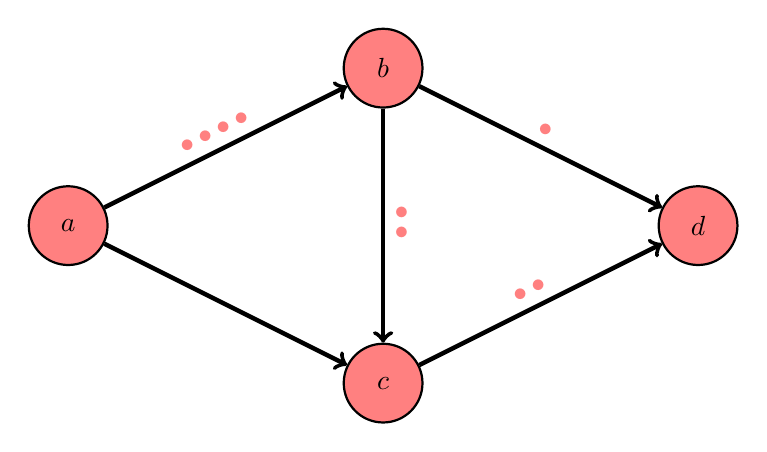
\begin{tikzpicture}
      \nodes{snapped}{snapped}{snapped}{snapped}
      \ab{arrow}{$\post \post \post \post$}
      \ac{arrow}{$\ $}
      \bc{arrow}{$\post \post$}
      \bd{arrow}{$\post$}
      \cd{arrow}{$\post \post$}
    \end{tikzpicture}
  \end{center}
\end{frame}

% Let's walk through the example presented in the paper. The red process
% records its state in the initial state. Then, the computation steps forward
% three events at which point, both channels and the blue state snapshot their
% states. The resulting snapshot is the one in a dashed box.
%
% If our snapshot algorithm produced a state that wasn't in our computation,
% what good is the snapshot? Well, there's a couple nice properties of our
% snapshot. First, notice that the snapshot is reachable from the initial
% state, and the final state is reachable from our snapshot.
\begin{frame}
  \begin{center}
    \scalebox{0.7}{
      \begin{tikzpicture}[xscale=3, yscale=1.5]
        \twotokensnap{}
        \pause
        \draw (sw01) rectangle (ne01);
        \pause
        \draw (sw03) rectangle (ne03);
        \pause
        \draw (sw05) rectangle (ne05);
        \pause
        \draw (sw07) rectangle (ne07);
        \pause
        \draw[dashed] (sw02) rectangle (ne02);
      \end{tikzpicture}
    }
  \end{center}
\end{frame}

\newcommand{\blackto}{\tikz{\draw[->, black, ultra thick] (0, 0) -- (0.5, 0);}}
\newcommand{\blueto}{\tikz{\draw[->, blue, ultra thick] (0, 0) -- (0.5, 0);}}
\newcommand{\greento}{\tikz{\draw[->, green, ultra thick] (0, 0) -- (0.5, 0);}}

% Moreover, there is a permutation of the computation that begins in the
% initial state, reaches the snapshot state, and terminates in the final state.
% In this example, our computation is blue, black, green. We can permute this
% to black, blue, green.
\begin{frame}
  \begin{center}
    \scalebox{0.7}{
      \begin{tikzpicture}[xscale=3, yscale=1.5]
        \twotokensnap{}
        \draw (sw01) rectangle (ne01);
        \draw (sw03) rectangle (ne03);
        \draw (sw05) rectangle (ne05);
        \draw (sw07) rectangle (ne07);
        \draw[dashed] (sw02) rectangle (ne02);
      \end{tikzpicture}
    }
  \end{center}
  \begin{gather*}
    \blueto \quad \blackto \quad \greento \\
    \blackto \quad \blueto \quad \greento
  \end{gather*}
\end{frame}

\begin{frame}{Snapshot Properties}
  Consider a computation $seq = S_0 e_0 S_1 e_1 \ldots S_\iota e_\iota \ldots
  S_\phi e_\phi \ldots S_n e_n$ where we initiate the snapshot algorithm in
  $S_\iota$ and the algorithm termiantes in $S_\phi$. Denote the snapshot state
  $S^*$.  We've seen that $S^*$ might not be equal to any $S_j$ for $\iota \leq
  j \leq \phi$. Howover, we can show that:
  \begin{enumerate}
    \item $S^*$ is reachable from $S_\iota$, and
    \item $S_\phi$ is reachable from $S^*$.
  \end{enumerate}
\end{frame}

\begin{frame}{Snapshot Properties}
  Even stronger, we can show that there exists a computation $seq'$ such that:
  \begin{enumerate}
    \item For all $i < \iota$, $i \geq \phi$, $e_i' = e_i$, and
    \item $(e_j', \iota \leq j < \phi)$ is a permutation of $(e_j, \iota \leq i
      < \phi)$, and
    \item there exists some $\iota \leq k \leq \phi$ such that $S^* = S_k'$.
  \end{enumerate}
\end{frame}

\begin{frame}{Stable Properties}
  Conceptually, a stable property of a distributed system $D$ is a property
  that is monotonically true. That is, once it becomes true, it remains true.

  \pause

  For example, the following are stable properties:
  \begin{itemize}
    \item Our one-token system has one token
    \item Our two-token system has two tokens
    \item Computation has terminated
    \item Computation is deadlocked
  \end{itemize}

  \pause

  Formally, a stable property $y$ is a predicate on the global states $S$ of a
  distributed system $D$. with the property that if $y(S)$ is true then $y(S')$
  is true for all states $S'$ reachable from $S$.
\end{frame}

% It's clear that the two-token system having two-tokens is a stable property
% because all states have two tokens!
\begin{frame}
  \begin{center}
    \scalebox{0.7}{
      \begin{tikzpicture}[xscale=3, yscale=1.5]
        \twotokensnap{}
      \end{tikzpicture}
    }
  \end{center}
\end{frame}

\begin{frame}{Stable Property Detection}
  We want to construct an algorithm that takes as input a distributed system
  $D$ and a stable property $y$, and outputs a boolean $b$ such that
  \[
    y(S_\iota) \implies b, \qquad b \implies y(S_\phi)
  \]
  Intuitively, if $b$ is true, then $y(S_\phi)$ is true. If $b$ is false, then
  $y(S_\iota)$ is false.

  \pause

  The algorithm itself is trivial:
  \begin{enumerate}
    \item Record a global state $S^*$
    \item Output $y(S^*)$
  \end{enumerate}
\end{frame}

% Looking at a system diagram, it should be clear why this is the case. If
% y(S*) is true, then by the definition of a stable property, y(S_phi) is true
% because S_phi is reachable from S*. Alternatively, if S* is not true, by the
% definition of a stable property, S_iota must not be true since S* is
% reachable from S_iota.
\begin{frame}
  \begin{center}
    \scalebox{0.7}{
      \begin{tikzpicture}[xscale=3, yscale=1.5]
        \twotokensnap{}
        \draw (sw01) rectangle (ne01);
        \draw (sw03) rectangle (ne03);
        \draw (sw05) rectangle (ne05);
        \draw (sw07) rectangle (ne07);
        \draw[dashed] (sw02) rectangle (ne02);
      \end{tikzpicture}
    }
  \end{center}
\end{frame}
